% Document preamble. Comment out for final figure! Footer too!
\documentclass[tikz, margin=5mm, dvipsnames]{standalone}
\usepackage{listings}
\usepackage{hyperref}
\usepackage{tcolorbox}
\usepackage{tikz}
\usetikzlibrary{shapes.geometric}
\usetikzlibrary{arrows.meta, arrows.spaced}
\usetikzlibrary{shapes.misc, positioning}
\usetikzlibrary{fit,backgrounds}
\usetikzlibrary{external}
\usetikzlibrary{calc}
%\tikzexternalize % activate!

%% Color definitions
\definecolor{recipecolor}{RGB}{210,169, 188}
\definecolor{rawcolor}{RGB}{235,235,235}
\definecolor{externalcolor}{RGB}{183,255,255}
\definecolor{calibcolor}{RGB}{255,250,216}
\definecolor{calproductcolor}{RGB}{185,184,237}
\definecolor{qcproductcolor}{RGB}{255,201,165}
\definecolor{sciproductcolor}{RGB}{197,219,183}

\definecolor{titlebackcolor}{RGB}{237,237,237}



%%% Recipe names: rectangles
\tikzstyle{recipe} = [%
  rectangle,
  minimum width=3.5cm,
%  minimum height=1cm,
  text centered,
  draw=black,
  fill=recipecolor]

%%% Raw frames
\tikzstyle{rawinput} = [%
  rounded rectangle,
  minimum width=3.5cm,
%  minimum height=1cm,
  text centered,
  draw=black,
  fill=rawcolor]

%%% Calib product
\tikzstyle{calibproduct} = [%
  minimum width=3.5cm,
  text centered,
  draw=black,
  fill=calproductcolor]

%%% QC product
\tikzstyle{qcproduct} = [%
  minimum width=3.5cm,
  text centered,
  draw=black,
  fill=qcproductcolor]

%%% External calibration files
\tikzstyle{extcalfile} = [%
  minimum width=3.5cm,
  text centered,
  draw=black,
  fill=externalcolor]

%%% Static calibration files
\tikzstyle{statcalfile} = [%
  minimum width=3.5cm,
  text centered,
  draw=black,
  fill=calibcolor]

%%% Science products
\tikzstyle{scienceproduct} = [
  minimum width=3.5cm,
  text centered,
  draw=black,
  fill=sciproductcolor]

%%% Connection
\tikzstyle{connection} = [%
  circle,
  inner sep=0pt,
  minimum size=0.2cm,
  draw=black,
  fill=black]  %% to be completed

%%% Products
\tikzstyle{product} = [%
  rounded rectangle,
  minimum width=4cm,
  minimum height=1cm,
  text centered,
  draw=black,
  fill=sciproductcolor]

%%% Arrows
\tikzstyle{arrow} = [%
  ultra thick,
  {-Stealth[scale=1.4]}]

\tikzstyle{match} = [ultra thick]
\tikzstyle{empty} = []

\newcommand{\recipebox}[2]{%
  \begin{tcolorbox}[%
    width=3.5cm,
    colbacktitle=titlebackcolor,
    coltitle=black,
    colback=recipecolor,
    adjusted title={\centering #1},
    halign=center]
    #2
  \end{tcolorbox}
}

\newcommand{\recipenotitlebox}[1]{%
  \begin{tcolorbox}[%
    width=3.5cm,
    colback=recipecolor,
    halign=center]
    #1
  \end{tcolorbox}
}


% ADDING NEW DEFINITIONS -------------------------------------------- start
\definecolor{listingbg}{gray}{0.95}
\definecolor{darkgreen}{rgb}{0.0, 0.7, 0.0}
\definecolor{darkblue} {rgb}{0.0, 0.0, 0.7}
\definecolor{cyan} {rgb}{0.0, 0.4, 0.4}
\definecolor{darkred}  {rgb}{0.7, 0.0, 0.0}
\definecolor{darkorange}{rgb}{1.0, 0.49, 0.0}
\definecolor{violett}{rgb}{255, 0, 255}
\definecolor{turq}{rgb}{0.0, 0.7, 0.8}
\definecolor{fits}{rgb}{0.4, 0.1, 1}


\makeatletter
\lstdefinestyle{RAWstyle}{%
  basicstyle=\ttfamily\color{black}%
  \lst@ifdisplaystyle\scriptsize\fi}

\lstdefinestyle{PARstyle}{%
  basicstyle=\ttfamily\color{black}%
  \lst@ifdisplaystyle\scriptsize\fi}

\lstdefinestyle{DRLstyle}{%
  basicstyle=\ttfamily\color{black}%
  \lst@ifdisplaystyle\scriptsize\fi}

\lstdefinestyle{RECstyle}{%
  basicstyle=\ttfamily\color{black}%
  \lst@ifdisplaystyle\scriptsize\fi}

\lstdefinestyle{QCstyle}{%
  basicstyle=\ttfamily\color{black}%
  \lst@ifdisplaystyle\scriptsize\fi}

\lstdefinestyle{TPLstyle}{%
  basicstyle=\ttfamily\color{black}%
  \lst@ifdisplaystyle\scriptsize\fi}

\lstdefinestyle{PRODstyle}{%
  basicstyle=\ttfamily\color{black}%
  \lst@ifdisplaystyle\scriptsize\fi}

\lstdefinestyle{EXTCALIBstyle}{%
  basicstyle=\ttfamily\color{black}%
  \lst@ifdisplaystyle\scriptsize\fi}

\lstdefinestyle{STATCALIBstyle}{%
  basicstyle=\ttfamily\color{black}%
  \lst@ifdisplaystyle\scriptsize\fi}
\makeatother

\makeatletter
\newcommand{\replaceunderscores}[1]{\expandafter\replace@underscores#1_\relax}

\def\replace@underscores#1_#2\relax{%
    \ifx \relax #2\relax
        #1%
    \else
        #1%
        \textunderscore
        \replace@underscores#2\relax
    \fi
}

\ExplSyntaxOn
% Generic \Smart@Item macro:
%   use \NEWRAW*{WHATEVER_THIS_IS} where hyperlinks are not needed (TOC, sections...)
%   and \NEWRAW{WHATEVER_THIS_IS} for a full hyperlink-enabled version in regular text and tikz figures
\NewDocumentCommand{\Smart@Item}{m m m O{dataitem}}{%
    \IfBooleanTF{#1}{%
        \texorpdfstring{\lstinline[style=#2style]!#3!}{\replaceunderscores{#3}}%
    }{%
        \hyperref[#4:\text_lowercase:n{#3}]{\lstinline[style=#2style]!#3!}%
    }%
}
\ExplSyntaxOff

% Raw FITS file: \NEWRAW{LM_SCI_RAW}
\NewDocumentCommand{\NEWRAW}{s m}{\Smart@Item{#1}{RAW}{#2}}
\NewDocumentCommand{\NEWPAR}{s m}{\Smart@Item{#1}{PAR}{#2}}
\NewDocumentCommand{\NEWDRL}{s m}{\Smart@Item{#1}{DRL}{#2}}
\NewDocumentCommand{\NEWREC}{s m}{\Smart@Item{#1}{REC}{#2}[rec]}
\NewDocumentCommand{\NEWQC}{s m}{\Smart@Item{#1}{QC}{#2}}
\NewDocumentCommand{\NEWTPL}{s m}{\Smart@Item{#1}{TPL}{#2}}
\NewDocumentCommand{\NEWPROD}{s m}{\Smart@Item{#1}{PROD}{#2}}
\NewDocumentCommand{\NEWREQ}{s m}{\Smart@Item{#1}{REQ}{#2}}
\NewDocumentCommand{\NEWEXTCALIB}{s m}{\Smart@Item{#1}{EXTCALIB}{#2}}
\NewDocumentCommand{\NEWSTATCALIB}{s m}{\Smart@Item{#1}{STATCALIB}{#2}}
\NewDocumentCommand{\NEWFITS}{s m}{\Smart@Item{#1}{FITS}{#2}}
\makeatother

%% Write DRL functions names like this: \hyperref[drl:function]{\DRL{function}}
\newcommand{\RAW}[1]{ \texorpdfstring{\lstinline[style=RAWstyle]!#1!}%
                                     {\replaceunderscores{#1}}}

%% Write DRL functions names like this: \hyperref[drl:function]{\DRL{function}}
\newcommand{\PAR}[1]{ \texorpdfstring{\lstinline[style=PARstyle]!#1!}%
                                     {\replaceunderscores{#1}}}

%% Write DRL functions names like this: \hyperref[drl:function]{\DRL{function}}
\newcommand{\DRL}[1]{ \texorpdfstring{\lstinline[style=DRLstyle]!#1!}%
                                     {\replaceunderscores{#1}}}

%% Write recipe names like this: \REC{metis_do_stuff}
\newcommand{\REC}[1]{ \texorpdfstring{\lstinline[style=RECstyle]!#1!}%
                                     {\replaceunderscores{#1}}}

%% Write QC parameters like this: \QC{QC_SOMETHING_OR_OTHER}
\newcommand{\QC}[1]{ \texorpdfstring{\lstinline[style=QCstyle]!#1!}%
                                    {\replaceunderscores{#1}}}

%% Write templates like this: \TPL{DARK_LM}
\newcommand{\TPL}[1]{ \texorpdfstring{\lstinline[style=TPLstyle]!#1!}%
                                     {\replaceunderscores{#1}}}

%% Write products like this: \hyperref[dataitem:some_thing]{\PROD{SOME_THING}}
\newcommand{\PROD}[1]{ \texorpdfstring{\lstinline[style=PRODstyle]!#1!}%
                                      {\replaceunderscores{#1}}}

%% Write requirements like this: \REQ{METIS-xxxx}
\newcommand{\REQ}[1]{\href{https://polarion.astron.nl/polarion/\#/project/METIS/workitem?id=#1}{\textcolor{brown}{#1}}}

%% external calib files
\newcommand{\EXTCALIB}[1]{ \texorpdfstring{\lstinline[style=EXTCALIBstyle]!#1!}%
                                          {\replaceunderscores{#1}}}

% static calib files
\newcommand{\STATCALIB}[1]{ \texorpdfstring{\lstinline[style=STATCALIBstyle]!#1!}%
                                           {\replaceunderscores{#1}}}

%% Write FITS keywords (and values) like this: \FITS{EXPTIME}
\newcommand{\FITS}[1]{ \texorpdfstring{\lstinline[]!#1!}%
                                      {\replaceunderscores{#1}}}


\begin{document}


% ADDING NEW DEFINITIONS -------------------------------------------- start
\definecolor{listingbg}{gray}{0.95}
\definecolor{darkgreen}{rgb}{0.0, 0.7, 0.0}
\definecolor{darkblue} {rgb}{0.0, 0.0, 0.7}
\definecolor{cyan} {rgb}{0.0, 0.4, 0.4}
\definecolor{darkred}  {rgb}{0.7, 0.0, 0.0}
\definecolor{darkorange}{rgb}{1.0, 0.49, 0.0}
\definecolor{violett}{rgb}{255, 0, 255}
\definecolor{turq}{rgb}{0.0, 0.7, 0.8}
\definecolor{fits}{rgb}{0.4, 0.1, 1}


\makeatletter
\lstdefinestyle{RAWstyle}{%
  basicstyle=\ttfamily\color{black}%
  \lst@ifdisplaystyle\scriptsize\fi}

\lstdefinestyle{PARstyle}{%
  basicstyle=\ttfamily\color{black}%
  \lst@ifdisplaystyle\scriptsize\fi}

\lstdefinestyle{DRLstyle}{%
  basicstyle=\ttfamily\color{black}%
  \lst@ifdisplaystyle\scriptsize\fi}

\lstdefinestyle{RECstyle}{%
  basicstyle=\ttfamily\color{black}%
  \lst@ifdisplaystyle\scriptsize\fi}

\lstdefinestyle{QCstyle}{%
  basicstyle=\ttfamily\color{black}%
  \lst@ifdisplaystyle\scriptsize\fi}

\lstdefinestyle{TPLstyle}{%
  basicstyle=\ttfamily\color{black}%
  \lst@ifdisplaystyle\scriptsize\fi}

\lstdefinestyle{PRODstyle}{%
  basicstyle=\ttfamily\color{black}%
  \lst@ifdisplaystyle\scriptsize\fi}

\lstdefinestyle{EXTCALIBstyle}{%
  basicstyle=\ttfamily\color{black}%
  \lst@ifdisplaystyle\scriptsize\fi}

\lstdefinestyle{STATCALIBstyle}{%
  basicstyle=\ttfamily\color{black}%
  \lst@ifdisplaystyle\scriptsize\fi}
\makeatother

%%% This file contains definitions of shapes and nodes used
%%% for a recipe workflow
%%% Author       : Oliver Czoske
%%% Created      : 2021-03-03
%%% Last Changed : 2021-03-03
%%% Changes:
%%%

\usetikzlibrary{
  shapes.misc,
  positioning,
  calc,
  arrows.meta}

%% All connecting lines have an arrow
\tikzset{
  connection_arrow/.style={->, >=Latex[open], thick}
}

%% Start and stop buttons (black disks, stop with ring)
%% These are pics, use as
%%         \pic (name) [above of=..] {picname};
\tikzset{
  start/.pic = {
    \node (-m) at (0, 0){};
    \filldraw [fill=black] (0, 0) circle (0.2);
  }
}

\tikzset{
  stop/.pic = {
    \node (-m) at (0, 0){};
    \node (-t) at (0, -0.3){};
    \filldraw [fill=black] (0, 0) circle(0.2);
    \draw[black] (0, 0) circle (0.3);
  }
}


%%%% Various boxes and their colours
%%%% These are nodes, use as
%%%% \node (name) [type, location]  {text};

\definecolor{stepcolor}{RGB}{210,169,188}
\definecolor{rawcolor}{RGB}{205,205,205}
\definecolor{externalcolor}{RGB}{183,255,255}
\definecolor{calibcolor}{RGB}{255,250,216}
\definecolor{calproductcolor}{RGB}{185,184,237}
\definecolor{qcproductcolor}{RGB}{255,201,165}
\definecolor{sciproductcolor}{RGB}{197,219,183}
\definecolor{framecolor}{RGB}{127,13,65}

\tikzset{
  %% template : the template(s) that trigger(s) the recipe
  template/.style={
    rectangle,
    draw=black,
    minimum width=4.0cm,
    minimum height=0.5cm,
    align=center
  },
  %% input : the input files
  input/.style={
    rectangle,
    fill=rawcolor,
    minimum width=4.0cm,
    minimum height=0.75cm,
%     text width=3cm,
    align=center
  },
  %% calib : calibration input
  calib/.style={
    rectangle,
    fill=calibcolor,
    minimum width=4.0cm,
    minimum height=0.75cm,
%     text width=3cm,
    align=center
  },
  %% external : external input
  external/.style={
    rectangle,
    fill=externalcolor,
    minimum width=4.0cm,
    minimum height=0.75cm,
%     text width=3.5cm,
    align=center
  },
  %% params : parameters
  params/.style={
    rectangle,
    draw=red,
    thick,
    minimum width=4.0cm,
    minimum height=0.75cm,
%     text width=3cm,
    align=center
  },
  %% redstep : a reduction step
  %%      ("step" is predefined and can't be used)
  redstep/.style={
    rectangle,
    rounded corners=0.2cm,
    fill=stepcolor,   %%% define colour!
    minimum width=4.0cm,
    minimum height=1cm,
%     text width=3cm,
    align=center
  },
  %% connection : connection to input or output
  connection/.style={
    circle,
    fill=black,
    minimum size=0.15cm,
    inner sep=0pt
  },
  %% sciproduct : a science product
  sciproduct/.style={
    rectangle,
    fill=sciproductcolor,
    minimum width=4.0cm,
    minimum height=0.75cm,
%     text width=3.5cm,
    align=center
  },
  %% calproduct : a calibration product
  calproduct/.style={
    rectangle,
    fill=calproductcolor,
    minimum width=4.0cm,
    minimum height=0.75cm,
%     text width=3.5cm,
    align=center
  },
  %% frame : frame around the recipe
  %% This is a path, use as
  %%    \draw [frame] (upper left) rectangle (lower right);
  frame/.style={framecolor, very thick, dashed}
}

%% Color definitions
\definecolor{recipecolor}{RGB}{210,169, 188}
\definecolor{rawcolor}{RGB}{235,235,235}
\definecolor{externalcolor}{RGB}{183,255,255}
\definecolor{calibcolor}{RGB}{255,250,216}
\definecolor{calproductcolor}{RGB}{185,184,237}
\definecolor{qcproductcolor}{RGB}{255,201,165}
\definecolor{sciproductcolor}{RGB}{197,219,183}

\definecolor{titlebackcolor}{RGB}{237,237,237}

%%% Recipe names: rectangles
\tikzstyle{recipe} = [%
  rectangle,
  minimum width=3.5cm,
%  minimum height=1cm,
  text centered,
  draw=black,
  fill=recipecolor]

%%% Raw frames
\tikzstyle{rawinput} = [%
  rounded rectangle,
  minimum width=3.5cm,
%  minimum height=1cm,
  text centered,
  draw=black,
  fill=rawcolor]

%%% Calib product
\tikzstyle{calibproduct} = [%
  minimum width=3.5cm,
  text centered,
  draw=black,
  fill=calproductcolor]

%%% QC product
\tikzstyle{qcproduct} = [%
  minimum width=3.5cm,
  text centered,
  draw=black,
  fill=qcproductcolor]

%%% External calibration files
\tikzstyle{extcalfile} = [%
  minimum width=3.5cm,
  text centered,
  draw=black,
  fill=externalcolor]

%%% Static calibration files
\tikzstyle{statcalfile} = [%
  minimum width=3.5cm,
  text centered,
  draw=black,
  fill=calibcolor]

%%% Science products
\tikzstyle{scienceproduct} = [
  minimum width=3.5cm,
  text centered,
  draw=black,
  fill=sciproductcolor]

%%% Connection
\tikzstyle{connection} = [%
  circle,
  inner sep=0pt,
  minimum size=0.2cm,
  draw=black,
  fill=black]  %% to be completed

%%% Products
\tikzstyle{product} = [%
  rounded rectangle,
  minimum width=4cm,
  minimum height=1cm,
  text centered,
  draw=black,
  fill=sciproductcolor]

%%% Arrows
\tikzstyle{arrow} = [%
  ultra thick,
  {-Stealth[scale=1.4]}]

\tikzstyle{match} = [ultra thick,-]
\tikzstyle{empty} = []

\newcommand{\recipebox}[2]{%
  \begin{tcolorbox}[%
%    width=3.5cm,
    hbox,
    colbacktitle=titlebackcolor,
    coltitle=black,
    colback=recipecolor,
    adjusted title={\centering #1},
    halign=center]
    #2
  \end{tcolorbox}
}

\newcommand{\recipenotitlebox}[1]{%
  \begin{tcolorbox}[%
%    width=3.5cm,
    hbox,
    colback=recipecolor,
    halign=center]
    #1
  \end{tcolorbox}
}



%%%%%%%%%%%%%%%%%% BEGIN DOCUMENT %%%%%%%%%%%%%%%%%%%%%%%%%%%%%%%%%%%%%%%%
\sffamily

%%% Picture: flow chart
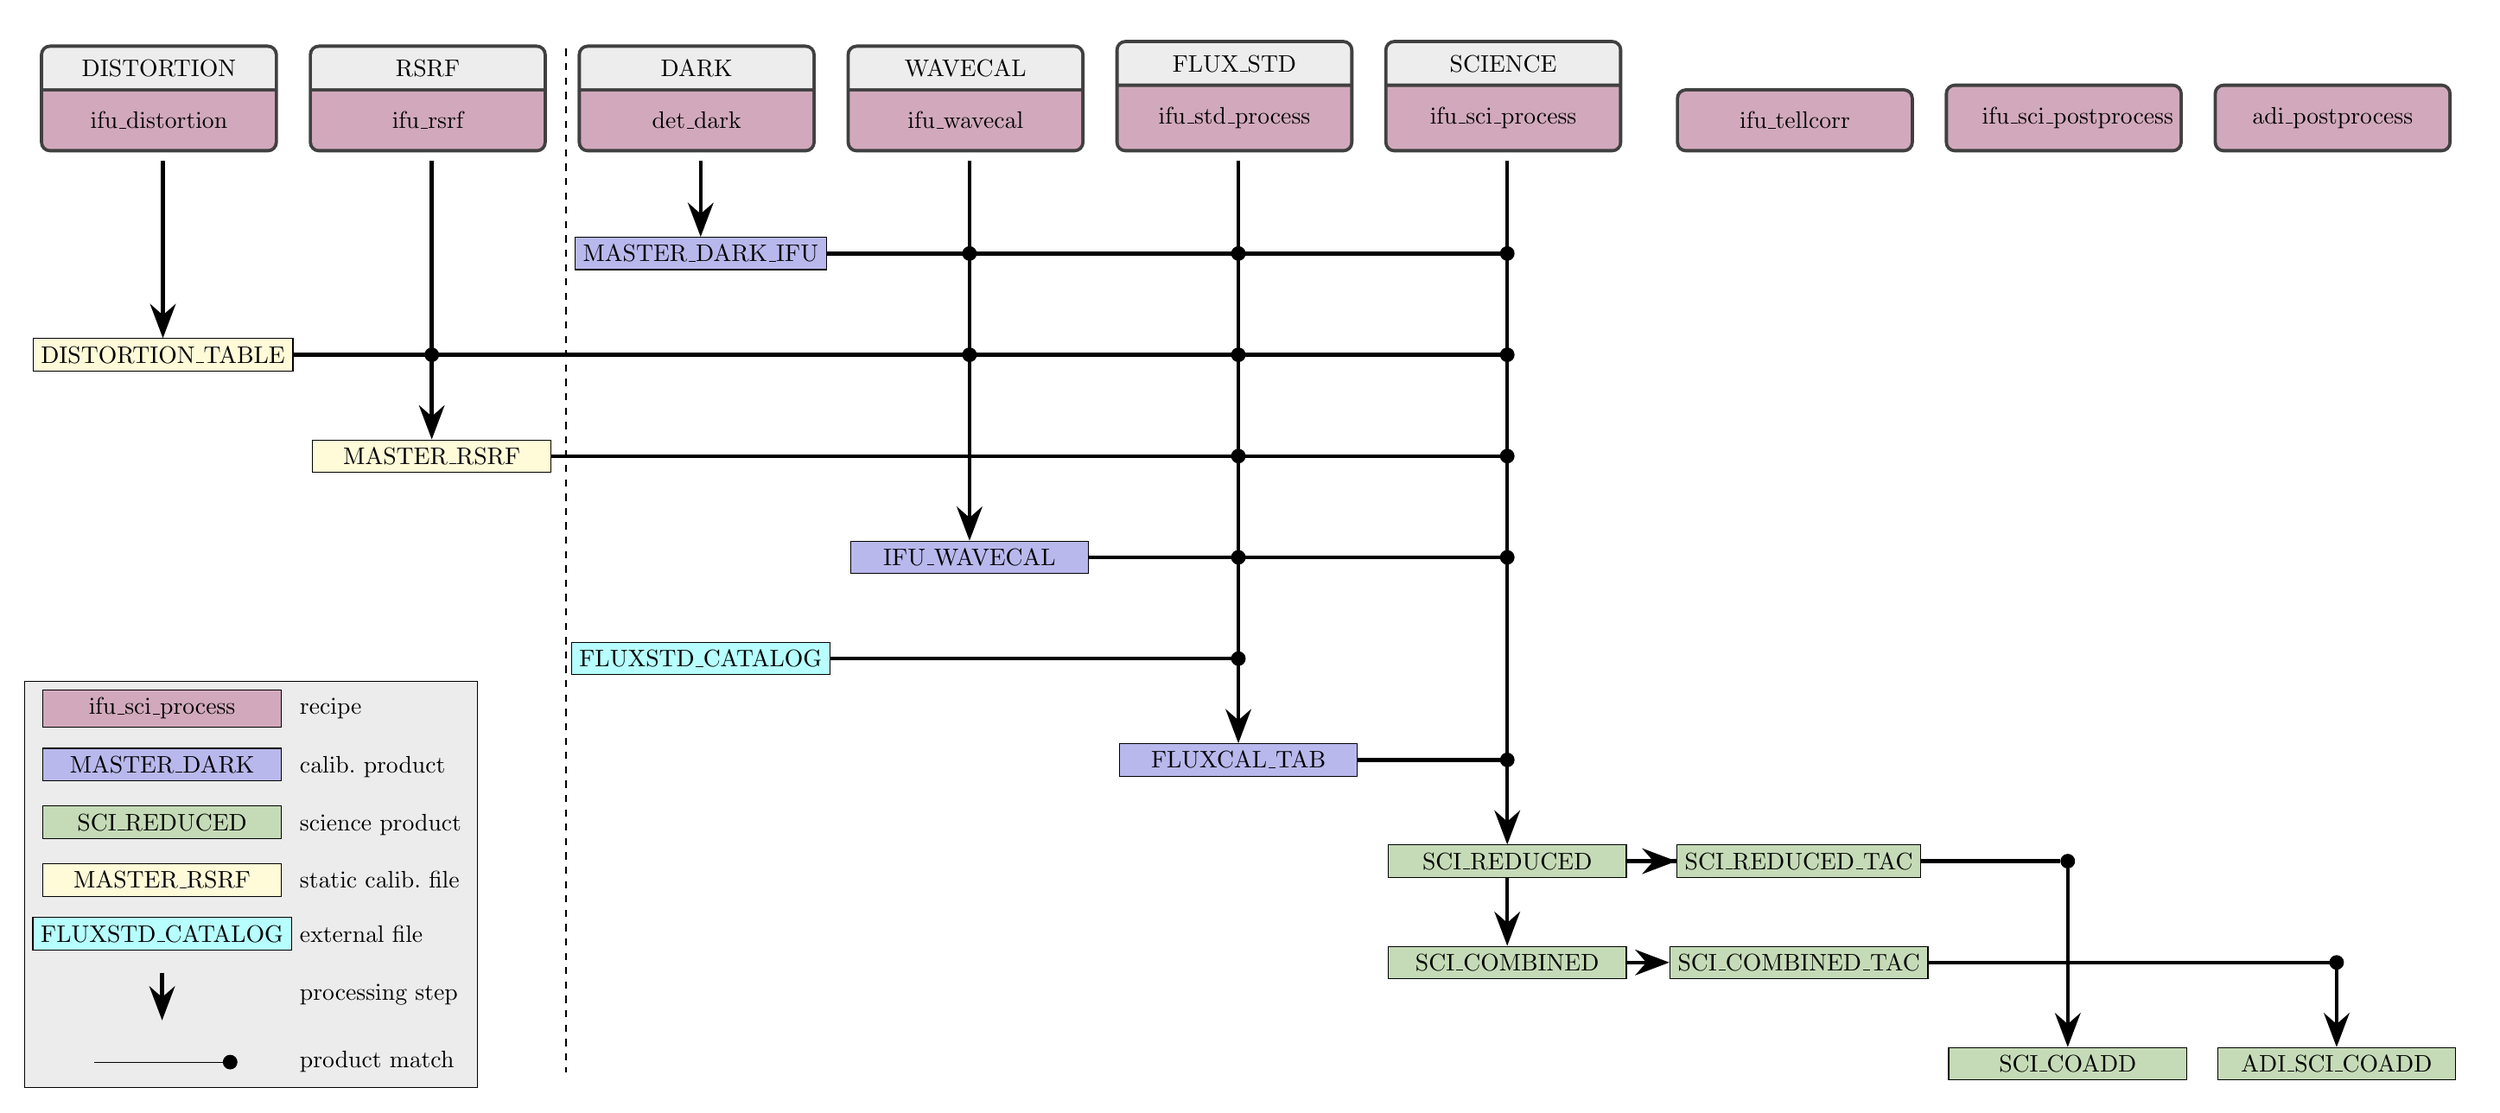
\begin{tikzpicture}[on grid=false, node distance=0.8cm]

  \matrix (recipes) [column sep=1mm, row sep=1cm]{
    % The matrix has columns
    % cal_*, dark_*, flat_*, std_*, sci1_*, sci2_*
    %
    % The matrix has rows
    % \  TBD

    % Row *_raw

    \node[above] (geom_raw){%
      \recipebox{DISTORTION}{ifu\_distortion}
    };
    &
    \node[above] (rsrf_raw){%
      \recipebox{RSRF}{ifu\_rsrf}
    };
    &
    \node[above] (dark_raw) {%
      \recipebox{DARK}{det\_dark}
    };
    &
    \node[above] (wcal_raw){%
      \recipebox{WAVECAL}{ifu\_wavecal}
    };
    &
    \node[above] (std_raw){%
      \recipebox{FLUX\_STD}{ifu\_std\_process}
    };
    &
    \node[above] (sci1_raw) {%
      \recipebox{SCIENCE}{ifu\_sci\_process}
    };
    &
    \node (space) [empty]{}; % horizontal spacing
    &
    \node[above] (tac_raw){%
      \recipenotitlebox{ifu\_tellcorr}
    };
    &
    \node[above] (sci2_raw){%
      \recipenotitlebox{ifu\_sci\_postprocess}
    };
    &
    \node[above] (adi_raw){%
      \recipenotitlebox{adi\_postprocess}
    };
    \\

    % Row *_dark
    \node (geom_dark)[empty]{};
    &
    \node (rsrf_dark)[empty]{};
    &
    \node (dark_dark) [calibproduct]{MASTER\_DARK\_IFU};
    &
    \node (wcal_dark)[connection]{};
    &
    \node (std_dark)[connection]{};
    &
    \node (sci1_dark)[connection]{};
    & &
    \node (tac_dark) [empty]{};
    &
    \node (sci2_dark)[empty]{};
    &
    \node (adi_dark)[empty]{};
    \\

    % Row *_geom
    \node (geom_geom) [statcalfile]{DISTORTION\_TABLE};
    &
    \node (rsrf_geom)[connection]{};
    &
    \node (dark_geom)[empty]{};
    &
    \node (wcal_geom)[connection]{};
    &
    \node (std_geom)[connection]{};
    &
    \node (sci1_geom)[connection]{};
    & &
    \node (tac_geom)[empty]{};
    &
    \node (sci2_geom)[empty]{};
    &
    \node (adi_geom)[empty]{};
    \\

    % Row *_rsrf
    \node (geom_rsrf) [empty]{};
    &
    \node (rsrf_rsrf) [statcalfile]{MASTER\_RSRF};
    &
    \node (dark_rsrf)[empty]{};
    &
    \node (wcal_rsrf)[empty]{};
    &
    \node (std_rsrf)[connection]{};
    &
    \node (sci1_rsrf)[connection]{};
    & &
    \node (tac_rsrf)[empty]{};
    &
    \node (sci2_rsrf)[empty]{};
    &
    \node (adi_rsrf)[empty]{};
    \\



    % Row *_wcal
    \node (geom_wcal)[empty]{};
    &
    \node (rsrf_wcal)[empty]{};
    &
    \node (dark_wcal)[empty]{};
    &
    \node (wcal_wcal) [calibproduct]{IFU\_WAVECAL};
    &
    \node (std_wcal)[connection]{};
    &
    \node (sci1_wcal)[connection]{};
    & &
    \node (tac_wcal)[empty]{};
    &
    \node (sci2_wcal)[empty]{};
    &
    \node (adi_wcal)[empty]{};
    \\

    % Row *_std
    \node (geom_std)[empty]{};
    &
    \node (rsrf_std)[empty]{};
    &
    \node (dark_std)[extcalfile]{FLUXSTD\_CATALOG};
    &
    \node (wcal_std)[empty]{};
    &
    \node (std_std)[connection]{};
    &
    \node (sci1_std)[empty]{};
    & &
    \node (tac_std)[empty]{};
    &
    \node (sci2_std)[empty]{};
    &
    \node (adi_std)[empty]{};
    \\

    % Row *_fcal
    \node (geom_fcal)[empty]{};
    &
    \node (rsrf_fcal)[empty]{};
    &
    \node (dark_fcal)[empty]{};
    &
    \node (wcal_fcal)[empty]{};
    &
    \node (std_fcal)[calibproduct]{FLUXCAL\_TAB};
    &
    \node (sci1_fcal)[connection]{};
    & &
    \node (tac_fcal)[empty]{};
    &
    \node (sci2_fcal)[empty]{};
    &
    \node (adi_fcal)[empty]{};
    \\

    % Row *_sci1
    \node (geom_sci1)[empty]{};
    &
    \node (rsrf_sci1)[empty]{};
    &
    \node (dark_sci1)[empty]{};
    &
    \node (wcal_sci1)[empty]{};
    &
    \node (std_sci1)[empty]{};
    &
    \node (sci1_sci1) [scienceproduct]{SCI\_REDUCED};
    & &
    \node (tac_sci1)[scienceproduct]{SCI\_REDUCED\_TAC};
    &
    \node (sci2_sci1)[connection]{};
    &
    \node (adi_sci1)[empty]{};
    \\

    % Row *_sci2
    \node (geom_sci2)[empty]{};
    &
    \node (rsrf_sci2)[empty]{};
    &
    \node (dark_sci2)[empty]{};
    &
    \node (wcal_sci2)[empty]{};
    &
    \node (std_sci2)[empty]{};
    &
    \node (sci1_sci2)[scienceproduct]{SCI\_COMBINED};
    & &
    \node (tac_sci2)[scienceproduct]{SCI\_COMBINED\_TAC};
    &
    \node (sci2_sci2) [empty]{};
    &
    \node (adi_sci2) [connection]{};
    \\

    % Row *_adi
    \node (geom_adi)[empty]{};
    &
    \node (rsrf_adi)[empty]{};
    &
    \node (dark_adi)[empty]{};
    &
    \node (wcal_adi)[empty]{};
    &
    \node (std_adi)[empty]{};
    &
    \node (sci1_adi)[empty]{};
    & &
    \node (tac_adi)[empty]{};
    &
    \node (sci2_adi)[scienceproduct]{SCI\_COADD};
    &
    \node (adi_adi)[scienceproduct]{ADI\_SCI\_COADD};
    \\
  };    % end matrix

  % dashed line separating daily procedure
  \node (t1) at ($(rsrf_raw)!0.5!(dark_raw)$){};
  \node (t2) at ($(rsrf_adi)!0.5!(dark_adi)$){} ;
  \draw [thick,dashed] ([yshift=4ex]t1.north) -- ([yshift=-0ex]t2.south);

  %% Connections
  \draw [arrow] (geom_raw) -- (geom_geom);
  \draw [arrow] (rsrf_raw) -- (rsrf_rsrf);
  \draw [arrow] (wcal_raw) -- (wcal_wcal);
  \draw [arrow] (dark_raw) -- (dark_dark);
  \draw [arrow] (std_raw)  -- (std_fcal);
  \draw [arrow] (sci1_raw) -- (sci1_sci1);
  \draw [arrow] (sci1_sci1) -- (sci1_sci2);
  \draw [arrow] (sci1_sci1) -- (tac_sci1);
  \draw [arrow] (sci1_sci2) -- (tac_sci2);
  \draw [arrow] (sci2_sci1) -- (sci2_adi);
  \draw [arrow] (adi_sci2) -- (adi_adi);

  \draw [match] (dark_dark) -- (sci1_dark);
  \draw [match] (rsrf_rsrf) -- (sci1_rsrf);
  \draw [match] (wcal_wcal)  -- (sci1_wcal);
  \draw [match] (geom_geom)  -- (sci1_geom);
  \draw [match] (sci1_sci1) -- (tac_sci1);
  \draw [match] (tac_sci1) -- (sci2_sci1);
  \draw [match] (tac_sci2) -- (adi_sci2);
  \draw [match] (dark_std)   -- (std_std);
  \draw [match] (std_fcal)  -- (sci1_fcal);

  %\draw [very thick,dashed] ($(raw_geometry.north)!0.5!(raw_dark.north)$) -- ++(270:15cm);

  %% Legend
  \matrix (legend) [draw, fill=gray!15, above right, row sep=0.3cm,
    column 1/.style={anchor=base},
    column 2/.style={anchor=base west}]
  at ([yshift=0cm]current bounding box.south west){%
    \node (leg_recipe) [recipe] {ifu\_sci\_process};
    & \node {recipe}; \\
    \node (leg_calproduct) [calibproduct] {MASTER\_DARK};
    & \node{calib.\ product}; \\
    \node (leg_sciproduct)[scienceproduct] {SCI\_REDUCED};
    & \node {science product}; \\
    \node (leg_statcalfile)[statcalfile] {MASTER\_RSRF};
    & \node {static calib.\ file};\\
    \node (leg_calfile)[extcalfile]{FLUXSTD\_CATALOG};
    & \node {external file}; \\

    \draw [arrow,fill=black] (0,0.4) -- (0,-0.3);  %% should be centred relative to column
    & \node {processing step}; \\

    \draw (-1, 0.5ex) -- (1,0.5ex) node [connection,yshift=0cm]{};
    & \node {product match}; \\
  };    %% end matrix (legend)

\end{tikzpicture}

%% Document footer. Comment out for final figure! Header too!
\end{document}
